\subsection{Definition}
\bigskip
\begin{figure}[!htb]
\begin{minipage}[t]{0.48\textwidth}
\vspace{-3cm}
In the first example (section \ref{bmt:heat_conduction_infinite}) there was a domain limited only by one side with a constant temperature at the boundary. The following problem shows the profile of a homogeneous and isotropic wall with a constant heat flow $q_{\mathrm{th}}$ on the left and a constant temperature $T_L$ on the right boundary (Fig.~\ref{fig-lhdw}). We consider diffusive heat transport on a two-side bounded domain.
\end{minipage}
\hspace{0.02\textwidth}
\begin{minipage}[t]{0.48\textwidth}
\centering
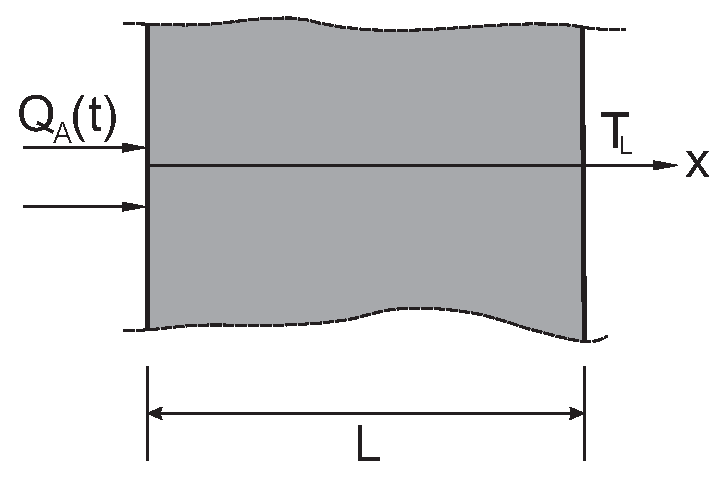
\includegraphics[scale=0.33]{PART_II/T/LHDW.eps}
\caption{\label{fig-lhdw}Heat conduction\\ through a wall}
\end{minipage}
\end{figure}

\vspace{-0.5cm}
\subsection{Solution}
\subsubsection{Analytical solution}

A solution for this problem can be found by solving the heat conduction equation \eqref{eqn:heat_conduction} using \textit{Fourier}'s method (see \cite{HaeSamVoi:92}).
\begin{equation}
\begin{split}
T(x,t) & = T_L + \frac{q_{\mathrm{th}}}{\lambda}(L-x) \\
& + 
\sum_{n=1}^{\infty} - \frac{8L}{(2n-1)^2\pi^2}\;\frac{q_{\mathrm{th}}}{\lambda} \cos{\frac{(2n-1)\pi x}{2L}}\;e^{(-\frac{(2n-1)^2\pi^2}{4L^2}\alpha\,t)}
\label{eqn:lhdw}
\end{split}
\end{equation}
with $T_L$ is the initial temperature, $Q_A$ is the constant heat source, $\lambda$ is the thermal conductivity and $\alpha$ is the heat diffusivity constant.

\begin{figure}[!htbp]
\centering
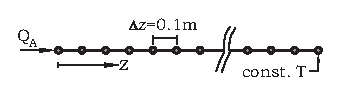
\includegraphics[width=0.5\textwidth]{PART_II/T/ms-lhdw.eps}
\caption{\label{fig-mslhdw}Boundary conditions and discretisation for the numerical model}
\end{figure}

\subsubsection{Numerical solution}

The numerical model consits of 40 line elements and 41 nodes along the $x$-axis (Fig.~\ref{fig-mslhdw}). The step size $\Delta z$ is set to $\unit[0.1]{m}$. On the left boundary a constant source term is set. The right side obtains a constant temperature condition.
%
Tab.~\ref{tab-ldhwp} shows the values of the used material properties. The heat diffusivity constant is $\alpha = \unit[3.1 \cdot 10 ^{-6}]{m^{2}}$/s. 

\begin{figure}[!htbp]
\centering
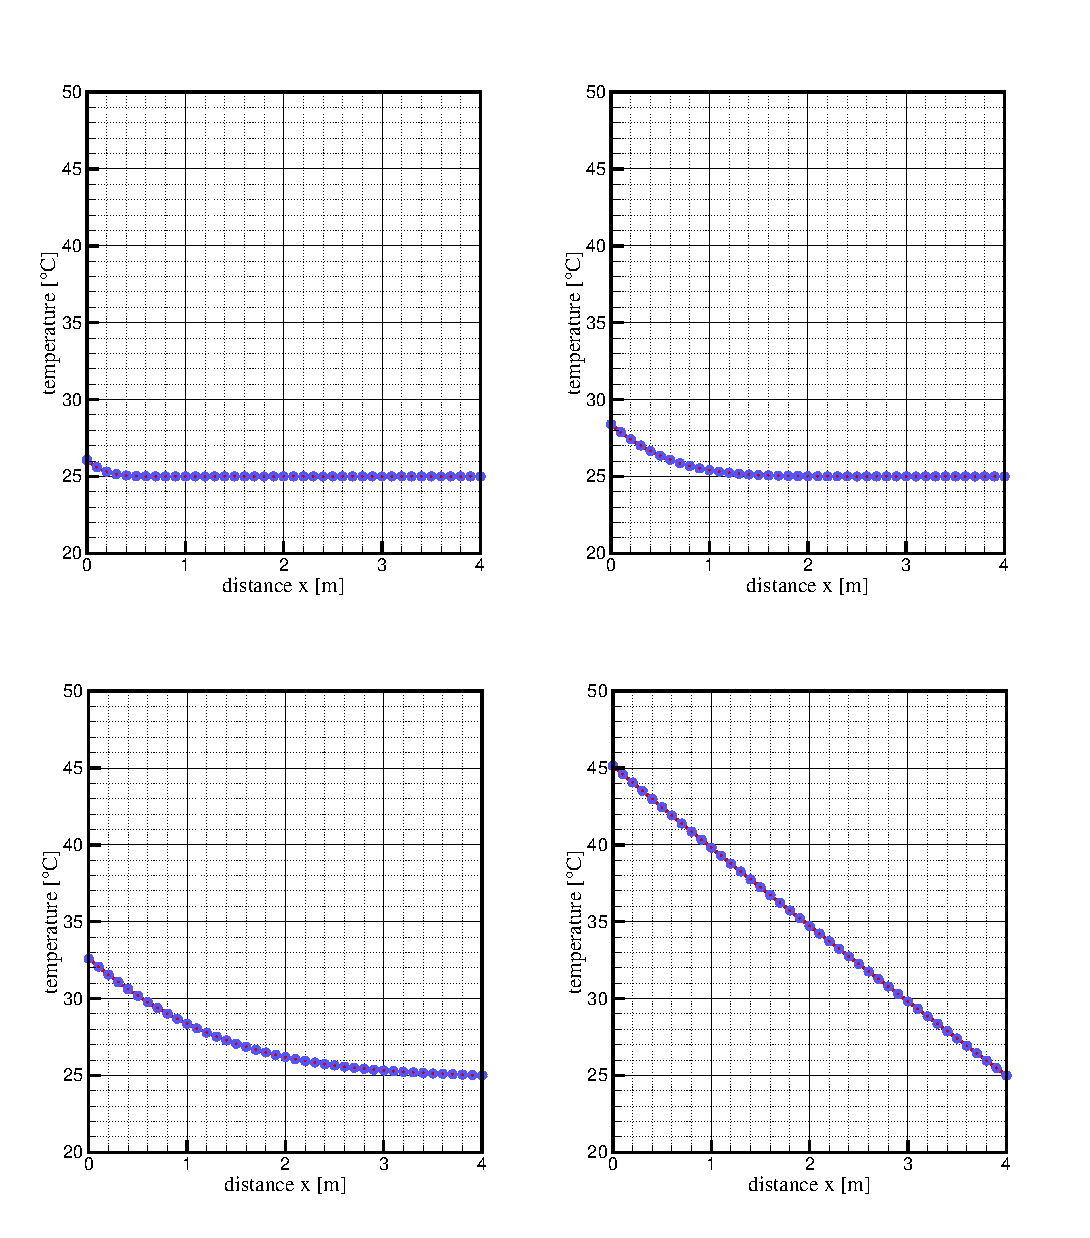
\includegraphics[width=0.8\textwidth]{PART_II/T/lhdw-all.eps}
\caption{Temperature distribution along the wall profile after 10.000, 100.000, 500.000 and 5.000.000 seconds (from top left to down right).}
\label{fig-lhdw-all}
\end{figure}

\subsection{Results}

The comparison of analytical and numerical solution is presented in Fig.~\ref{fig-lhdw-all}. It shows the distribution of the temperatue along the profile of the wall. Due to the thickness of the wall, the heat transport takes very long, after 5$\times 10^6$ seconds ($\approx$ 58 days) the temperature distribution becomes staedy-state.
%

\begin{table}[!htbp]
\caption{\label{tab-ldhwp}Material properties.}
\begin{center}
\begin{tabular}{llrr}
\toprule
Symbol & Parameter & Value & Unit \\
\midrule
$q_{\mathrm{th}}$ & Heat source & $\unit[30]{}$   &  ${W \cdot m^{-2}}$ \\			
$T_L$ & Initial temperature	  & $\unit[25]{}$   & ${^{\circ}C}$ \\
$L$   & Wall thickness          & $\unit[4]{}$    & ${m}$ \\
$\rho$& Density of the solid	  & $\unit[2000]{}$ & ${kg \cdot m^{-3}}$ \\			
$c$   & Heat capacity           & $\unit[900]{}$  & ${J \cdot kg^{-1} \cdot K^{-1}}$ \\
$\lambda$& Thermal conductivity & $\unit[5.5]{}$  & ${W \cdot m^{-1} \cdot K^{-1}}$ \\
\bottomrule
\end{tabular}
\end{center}
\end{table}

%\clearpage
